% Template for 61st conference for non-peer-reviewed articled
\documentclass[convention]{aesconf}

% Graphics path
\graphicspath{{./}{figures/}}

% UTF-8 encoding is recommended but use one that works for you.
\usepackage[utf8]{inputenc}

% Highly recommended package for better looking text automatically.
\usepackage{microtype}

% Natbib is used for more control on citations. You can use other moderd
% bibliography packages but please try to match the provided style.
\usepackage[numbers,square]{natbib} 


% These are useful for different purposes.
\usepackage{color}
\usepackage{url}


% The full title of the paper
\title{Audio Source Localization as an Input to Virtual Reality Systems}

% Put the authors in order here. The number in brackets define the corresponding affiliation.
\author[1]{Agneya A. Kerure}
\author[1]{Jason Freeman}

% Affiliations go here
\affil[1]{Georgia Institute of Technology}

% Correspondece should include the corresponding author's name and e-mail address
\correspondence{Agneya A. Kerure}{kerure.agneya@gatech.edu}

% These are used for headers. Anything that fits is okay. Please use proper punctuation.

% If there are many authors, please use the form "First author et al."
\lastnames{Kerure and Freeman}

% Short title should describe your topic but not be too long.
\shorttitle{Audio Source Localization in VR}


% This is required and draws the top title
% AES top title. A little bit volatile but should work for now.
\savebox{\AEStop}{%
	\begin{minipage}{\textwidth}%
		\rule{\textwidth}{1.5pt}\\%
		\\%
		\begin{minipage}[c][\iftoggle{convention}{3.2cm}{3.7cm}][t]{0\textwidth}%
			
\includegraphics[width=20mm]{aeslogo.pdf}%
		\end{minipage}%
		\begin{minipage}{\textwidth}%
			\sffamily%
			\begin{center}%
				\LARGE Audio Engineering Society\\%
				\iftoggle{e_brief}{%
				\hspace{3mm}\fontsize{36}{38pt}\selectfont Convention e-Brief \AESEBriefNumber\\%
				}{%
				\iftoggle{convention}{%
				\fontsize{36}{38pt}\selectfont Convention Paper\\%
				}{%
				\fontsize{36}{38pt}\selectfont Conference Paper\\%
				}}%
				\vspace{0.2cm}%
				\large Presented at the \AESConferenceNumber \iftoggle{convention}{Convention\\}{Conference on\\}%
				\iftoggle{convention}{}{\AESConferenceTopic\\}%
				\AESConferenceDate, \AESConferenceLocation%
			\end{center}%
		\end{minipage}\\%
		\vspace{0.2cm}\\%
		\begin{minipage}{\textwidth}%
			\rmfamily\itshape\small	\AESLegalText%
		\end{minipage}\\%
		\\%
		\rule{\textwidth}{1.5pt}%
	\end{minipage}%
}


\begin{document}


\twocolumn[
\maketitle % MANDATORY! 

\begin{onecolabstract}
This paper details an effort towards incorporating audio source localization as an input to virtual reality systems, focusing primarily on games. The goal of this research is to find a novel method to use localized live audio as an input for level generation or creation of elements and objects in a virtual reality environment. The paper discusses the current state of audio-based games and virtual reality, and details the design requirements of a system consisting of a circular microphone array which can be used to localize the input audio. The paper also briefly discusses signal processing techniques used for audio information retrieval and introduces a prototype of an asymmetric virtual reality first-person shooter game as a proof-of-concept of the potential of audio source localization for augmenting the immersive nature of virtual reality.
\end{onecolabstract}
]

\section{Introduction}
Audio and music have historically been a passive part of video games. Soundtracks that accompany video games have been used to captivate the player's attention and incorporate a sense of realism and emotion into the game, but have rarely been an active part of the game-play mechanism until recently.

Music driven games started out in the form of rhythm-based games where the player's sense of rhythm is challenged. These games started out in Japan as electromechanical arcade games where users would press buttons in rhythm to score more points. As time progresses, the required rhythm gets more complicated and increases in speed. Games such as Guitar Hero\footnote{https://www.guitarhero.com} and Dance Dance Revolution \footnote{https://www.ddrgame.com} typically involve players in performing certain actions in the form of a dance or pressing buttons in a sequence. Virtual reality-based rhythm games work in a similar manner but rely on handheld controllers or motion trackers to interact with the rhythmic elements of the game.

Apart from rhythm, there are games such as Yasuhati \footnote{https://www.yasuhati.com} which use audio from the user as a core mechanism of game-play. These typically rely on features like volume and pitch to control some aspects of the game. Speech recognition has also been used as an input modality, typically for performing certain actions in the game or to control user interfaces in games.
The use of audio and its properties as an input to games has been very minimal and with the advancement in gaming technology and signal processing prowess of computers, an exploration of these possible real-time interactions is warranted. In virtual reality specifically, the potential of localized audio and it's properties to be used meaningfully in game-play is immense. In this paper, we explore the use of audio source localization as an input to virtual reality.

An important question to consider would be - "Why use audio for localization?". There are other ways to locate objects and people in a vicinity around a person which include computer vision, infrared tracking, and even GPS. The advantage audio offers is the ability to process the received signal and get vast amounts of information from it, such as timbral and temporal properties along with the direction of arrival, which can be used in different ways in the game with minimal hardware costs.
Virtual reality offers a paradigm which enables interactions in 360$^\circ$. To fully utilize this paradigm, the proposed audio localization system for VR involves a circular microphone array which localizes sounds in 360$^\circ$. This enables truly immersive interactions.

\section{Background}

Sound properties such as pitch and sound pressure level have been used as a method of input in games for immediate, real-time control, as discussed by Igarashi and Hughes\cite{Igarashi:2001:VSU:502348.502372}. Through prototyping, they explore various interaction methods based on voice such as control by continuous voice, rate based continuous control by pitch and discrete parameter control by tonguing\cite{Igarashi:2001:VSU:502348.502372}. H{\"a}m{\"a}l{\"a}inen et. al. \cite{hamalainen2004musical} have examined the use of singing voice pitch to control a game so that the player learns to control his/her voice and sing correctly with the help of immediate graphical feedback. It was found that using singing as a method of control was a good way to teach children to sing correctly in pitch. It was also found that background music affected the pitch detection mechanism being used in their game and suggest the use of acoustic noise cancellation to prevent this behavior \cite{hamalainen2004musical}. Harada et. al. \cite{harada2011voice} developed a "Voice Game Controller" that augmented traditional speech-based input methods with non-speech voiced input methods that made computer games originally designed to be played with a keyboard and mouse setting playable using voice only. It was found that their prototype controller greatly expanded the scope of games that could be played hands-free using just voice, to include games that were difficult or impractical to play using previous speech-based methods \cite{harada2011voice}.

Mobile-based games have also used audio as an input to control certain aspects of the game. Chicken Scream \footnote{http://www.perfecttapgames.com} is a mobile game in which the user controls the main character by shouting and screaming. The louder the shout, the faster the character moves. Modulation of volume is used as a mechanism to overcome in-game obstacles.

Audio-only games refer to games which can only be played and perceived through sound and acoustics. They were initially developed for the visually impaired community but have huge potential for mobile and multi-player gaming \cite{rober2005playing}. Although these games are limited in the amount of information which can be conveyed to the player, they also have a few advantages over conventional games, such as increased degree of spatial freedom, no necessity of screens and other costly equipment depending upon the game, lower computational complexity and hence less latency, making them perfectly suited for mobile gaming. It has also been suggested that audio-mostly games could be more immersive than visual video games since the lack of visual information will provide more room for players to use their imagination\cite{liljedahl2007beowulf}. The development of games for visually impaired players has produced several studies investigating audio-based gaming for genres such as action\cite{Atkinson:2006:MMA:1183316.1183321} and mystery/adventure \cite{drewes2000sleuth}.

There are many games in the virtual reality category which use music as an input to generate in-game content. Audioshield\footnote{http://audio-shield.com} and Rockband VR\footnote{http://www.rockbandvr.com} are the most important examples of this genre. These typically use predetermined times derived from the music being played to create cues in the forms of game-objects.

There are not many games which utilize the spatial nature of virtual reality which has the potential to use localized interactions. This paper explores the use of audio source localization i.e. the direction from which a sound arrives as an input to virtual reality games. This provides a new method of interaction which uses the spatial nature of virtual reality in a unique way. 

\section{Interaction Design}
The nature of the application which uses the location of an audio source in a virtual reality can be varied - games, test simulations, training environments and social interactions are just a few possibilities. This paper will explore the avenue of game design using the provided source localization and other audio feature data.

The proposed method of interaction using audio source localization brings local real-time interaction in the virtual space closer to naturalistic interactions rather than interactions through only buttons and controllers. This introduces the opportunity to design and develop customized in-game dynamics between the players and the game environment in the physical and virtual space. While most mappings between features and in-game elements should be 1:1 to maintain understandability, using the position and movement of multiple people with the ability to control the digital realm brings many possibilities. There is potential for the use of continuous movement of the non-VR player while making noises to control or move game-objects, the use of audio properties to change in-game environment or visuals to not only to make the game more visually appealing but to also make it challenging for the VR player to play the game. High-level features could also be extracted from the sounds generated by the non-VR player and be used to convey meta information about the state of the game. The nature of game-play could be dictated by the non-VR player, for example, if player generated sounds which are classified as tense in nature are sustained for a long period of time, the game-play could get aggressive and volatile.

A major use of the proposed interaction system is the instantiation of game-objects based on the direction of incoming audio. These game-objects can behave in a number of different ways. The instantiated game-objects can follow a predetermined path for different directions of arrival. This could be used for puzzle games such as Keep Talking and Nobody Explodes \footnote{https://www.keeptalkinggame.com}, which would require the user to solve puzzles or mazes using sound and movement. A second approach could be for the instantiated objects to follow a particular game object or direction which could require the use of speakers in multiple locations in the physical play space. The third and easiest approach would be to only instantiate stationary objects based on the direction of arrival. This approach could be more useful for certain non-game applications such as simulation, analysis, and test environments. 

There is a need to understand and meaningfully map the varied set of features available through localized audio. It would be easy to get lost in the information available through this new method of interaction. It is very important to keep the mapping of these features to the elements of game-play easy to understand and learn. A game should provide continuous satisfaction and feedback to the players for their actions. There must be a balance between the ease of use of the designed system of interaction and it's sophistication to keep the player engaged for an extended period of time.

To test the use of the features made available by localized audio, a prototype first-person shooter game was developed using the system described in the next section.

\section{System}  

A general overview of the proposed system is provided in Figure 1. A circular microphone array mounted on the VR headset is used to capture sound in the form of speech, noise and music from different locations around the microphone. This audio data is used not only to extract audio features but also the direction of arrival of the audio to the microphone. Audio features such as pitch, loudness, and keywords are extracted and are used to affect game-play in a perceptually meaningful way. This means that the data extracted is mapped to certain aspects of the game where this mapping is easily understood and used by the players affect the game in real-time. 

\begin{figure}[ht!]
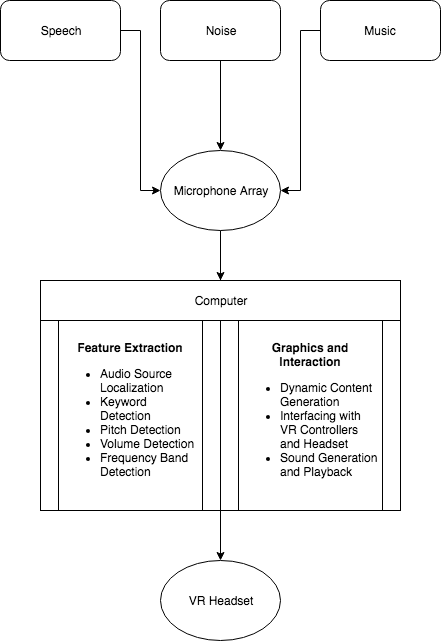
\includegraphics[width=\linewidth]{System_Diagram}
\caption{System Overview}
\label{auravr} %% The label
\end{figure}

For pitch detection, the system uses the time-domain based autocorrelation approach. Here the input signal is divided into short frames and the period of a frame is estimated by computing the autocorrelation functions. In this method, the autocorrelation sequence of each frame of the input audio is determined and the time lag corresponding to the strongest peak is used to determine the fundamental pitch period. This technique is most effective in the mid- to low-frequency range and thus has been popular in speech recognition applications. The autocorrelation function is represented by: 

\[ 
[R] (t)  = \int_{i=-{\infty}}^{\infty} S_i^*(\tau) S_i(t+\tau) \delta \tau \]

Octave errors are common in autocorrelation based pitch detectors. This happens, particularly with low-quality microphones. Fortunately, the prototype game developed is not affected by such errors as accurate note tracking is not required.

The loudness of the sound is calculated by extracting the root mean square of the signal over a frame of samples. 

\[
    x_{rms} = \sqrt{ \frac{1}{n}\ (x_1^2 + x_2^2 + ... + x_n^2) }
\]

Certain aspects of the game depend on the grouping of frequency bands together. This is done in Unity3D using inbuilt FFT functions which turns input audio into frequency and amplitude components. The audio samples are then grouped together according to their frequencies into 2 "bands" - one containing bass frequencies between 60-200 Hz and one containing mid to high range frequencies between 300-1000 Hz.

\section{Prototype}
First-person shooter games, which involve the user in a weapon-based combat environment, made a compelling use case for the proposed system as it would require increased concentration from the user, who would have to anticipate a target object based on their own sense of hearing, thereby increasing their involvement and immersion in the game. A prototype game was developed to test the proposed interaction method.

The system included a microphone array for the capture of audio to estimate the incident audio angle. The localization of sounds is being done by the ReSpeaker Microphone Array\footnote{https://www.seeedstudio.com} which uses its XMOS XVSM-2000 DSP chip to perform functions like audio source localization through beamforming, vocal activity detection, and dereverberation. These functions are built into the microcontroller and are easily accessible on a Windows machine using the HIDAPI protocol. It has a small form factor along with an LED ring to show the direction of arrival it detects.

The game was developed in Unity3D for the HTC Vive VR headset. The system uses an application developed using the JUCE framework \footnote{https://www.juce.com} to process the input audio from the microphone. This is because Unity does not natively support multichannel audio input for processing. The audio back-end communicates with Unity via Open Sound Control \cite{wright2005open}. The speech recognition used in the system is accomplished using the Microsoft Speech Recognition tool for Unity \footnote{https://developer.microsoft.com}. 

A prototype two player shooting game was designed to utilize audio localization as an input. This utilized a typical asymmetric VR game mechanism in which one player wears the VR headset and the other utilizes a secondary screen to view and play the game. The objective of the game for the VR player is to survive attacks from the second player for as long as possible. The objective for the second player is to defeat the VR player by attacking using his voice - by speaking certain commands which launch projectiles towards the VR player. The VR player can shoot at or protect himself from these incoming projectiles using the hand-held HTC Vive controllers, utilizing a bow-and-arrow, and shield mechanism. The projectiles have properties attached to them which are controlled by the properties of the voice of the second player. The pitch of the voice is mapped to the y-axis location i.e the height at which the projectile flies, the volume determines the size and damage of the projectile, and the location of the player with respect to the microphone array determines the origin of the projectiles relative to the position of the speaker. The non-VR player moves around the VR player, "shouting" projectiles towards the VR player which cause in-game damage.

\subsection{Mechanics and UI}

\begin{figure}[ht!]
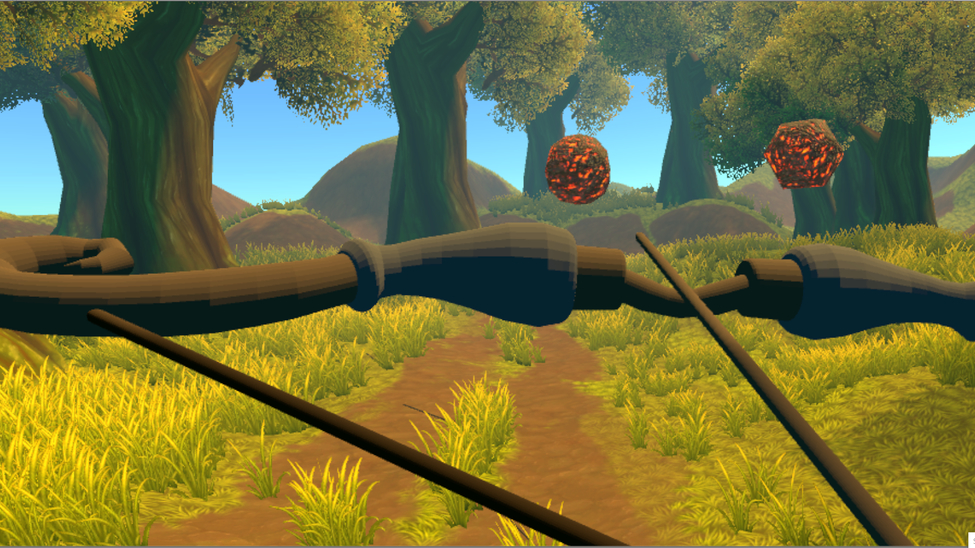
\includegraphics[width=\linewidth]{1}
\caption{In-Game VR Graphics}
\label{auravr} %% The label
\end{figure}


\begin{figure}[ht!]
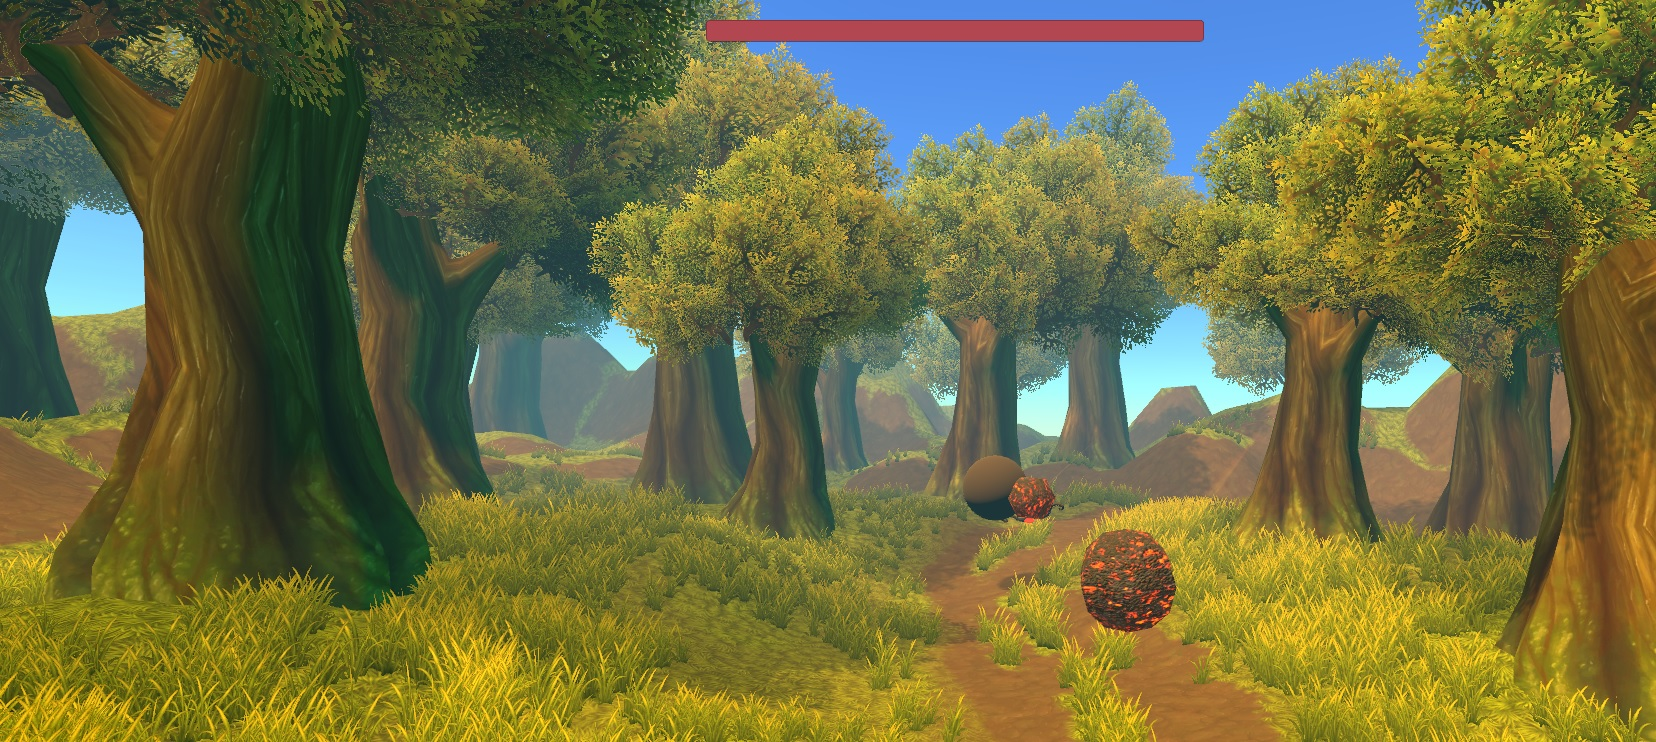
\includegraphics[width=\linewidth]{3}
\caption{Secondary Display (Non VR)}
\label{auravr2} %% The label
\end{figure}

The VR player uses hand-held controllers to shoot at targets using a bow-and-arrow mechanism. The right-hand pulls the arrow back keeping the "Trigger" button pressed. To release the arrow, the trigger button is released. The non-VR player utilizes voice commands to play the game. The command "Strike" instantiates a target fireball which deals damage to the VR player if hit. The location of the targets depends on the physical location of the non-VR-player while shouting the command. The volume of the speaker determines the size, health, and damage done by the instantiated targets.

After the targets are created, the non-VR player can change their height by speaking in different pitches. The higher the pitch, the more the Y-deviation of the instantiated target in motion. The health of the opponent is visible on the monitor along with his position and the trajectories of the targets.The frequency detected by the microphone is displayed to the right of the opponent health bar. This pitch determines the height at which the targets fly.

As soon as the VR player is defeated, the players would ideally switch roles to compete to see who would last the longest as the VR player and who could best utilize the interaction to beat the opponent quickly.

\subsection{Feedback and Discussion} 
The game has undergone several iterations of prototyping based on informal playtesting with 10 participants. The playtesters were intrigued by the asymmetric nature of gameplay and naturalistic interaction in the real and virtual space. While there was a considerable learning curve to understand the audio based controls of the game and the need for movement, most of the feedback was positive, with people getting excited about the potential of this technology in the world of audio-based interactive games and software.

As for the design of the game, it was noticed that there was a visible imbalance between the in-game skills required by the VR player and the non-VR player who uses his voice. There was very little skill required by the non-VR player to win the game as he could just keep saying the keyword to generate a large number of projectiles towards the VR player. This helped realize the need to limit the number of projectiles created. There was also a need to restrict potential projectile spawn points so that it is easier for the players to understand the game and how movement was actually correlated to the spawning of the projectiles. 
To increase the skill required and the involvement of audio localization, the non-VR player was given the ability to control the path of the projectile towards the VR player by singing and changing the pitch of his voice - the pitch was directly correlated to the y-axis displacement from the original trajectory. This also provided for a fun experience for the VR user as he now had to try and guess where the opponent would take his projectile and shoot at it. There was also an aspect of the usage of real world skills by the VR player by using hearing abilities to localize audio and anticipate the location from which the opponent may shoot. This also added to the amalgamation of real and virtual world interactions required in the game.

An important decision taken was to use a real-time keyword detection library over a trained classifier which provided less latency but compromised on accuracy. A classifier would serve the needs for this game better but due to limitations in time, it was not implemented. The Microsoft keyword detection software was easy to implement and does the job decently with acceptable latency.

There was an understandable bias towards wanting to be the VR player rather than the one trying to attack using the microphones due to the truly immersible nature of virtual reality. Future enhancements to the audio localization system will attempt to bridge this preference gap by increasing the functionality and intuitive ease of use for the non-VR player.

Real-time audio source localization, information extraction, and keyword detection have varying amounts of latency associated with them. Meaningfully mapping this information to instantiated game objects so that it is understood by the players is a challenge which should be addressed while designing for this system.

The in-game audio is highly affected by the acoustic nature of the proposed system. A system which utilizes loudspeakers is bound to produce sounds which will be considered as noise in the audio source localization system, thus greatly reducing the accuracy of localization. It is very important to optimize speaker settings in order to utilize this method of interaction for games. It is ideal to use headphones during game-play to minimize the possibility of noise affecting the system.

\section{Conclusion}
This paper proposes a system which involves audio source localization and signal processing to provide inputs to a virtual reality environment. The use of this system in a prototype game as a proof-of-concept has been discussed, and the hardware and software requirements of the system were mentioned. Learning from the informal playtesting feedback, the prototype game was an engaging and intriguing experience making the case for a new method of interaction to achieve dynamic real-time control over a virtual environment through localized audio.

\bibliographystyle{jaes}

% Reference to bibliography file.
\bibliography{refs}


\end{document}